\documentclass[../main.tex]{subfiles}

\begin{document}

\section{Platform-Agnostic Bytecode}
\subsection{Definition}

A Platform-Agnostic Bytecode (PAB) is a bytecode that follows those two main principles:

\begin{itemize}
    \item Turing Completeness
    \item Support for tooling that makes it executable on every machine
\end{itemize}

A bytecode like this ideally is designed to be executed on a virtual machine that follows general patters. This design should make easier the compilation to another real machine's bytecode. Examples of real architectures with specified bytecode are AMD and Intel with x86 or ARM with aarch64. % TODO: check this last sentence

\subsection{Execution}

PABs require multiple phases of Compilation, the first one is encountered when you want to compile your High-Level language to the PAB using a Cross-Compiler. Once you have the arbitrary PAB code, you should be able to run it on every machine using another compiler that will create the final executable code.

Re-compiling is not the only way to execute a PAB, another common solution is to implement a Virtual Machine (VM) able to run arbitrary PAB code interpreting it.

\subsection{Key features}

Every bytecode, ideally, can become a PAB if tools to make it runnable to different machine exist, then there are some metrics to define which one is the better than other, example of metrics are:

\begin{description}[style=nextline]
  \item[Hardware Independence]
        A bytecode can't be a PAB if tightly related to specific hardware. A PAB can be defined as such if there is no direct connection between bytecode and hardware, the only exception is if the relations require only a little overhead for the execution on different hardware.
  \item[Sandboxing]
        The machine used to execute the PAB is defined as \textit{embedder}. The embedder will execute arbitrary code, possibly malicious, and avoiding any security problem is the main goal, a sandboxed environment is the solution. The execution in a different environment makes almost impossible to compromise the embedder from the PAB code. Implemening a proper sandboxed environment is embedder dependent but a PAB can be more or less suitable for this feature.

        \begin{figure}[h]
          \centering
          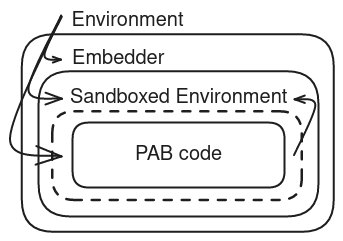
\includegraphics[width=0.4\linewidth]{sandboxed_env.png}
          \caption{Sandboxing graphic example}
          \label{fig:Sandboxing graphic example}
        \end{figure}

  \item[Efficiency]
        The efficiency of a PAB has a lot of meaning, it could be:

        \begin{itemize}
          \item Compiling High-Level Language to the PAB
          \item Execution of the PAB, it could be the compilation to the final bytecode and then execution, the interpretation or more complex solutions
        \end{itemize}

        Generally the first is not really related to the PAB, but more on the used tools (examples gcc, rustc, etc.). The execution efficiency is the real deal, how fast a PAB can be executed on a machine is crucial.
  \item[Tool Simplicity]
        The easiness of compiling an High-Level language and the executing the PAB is very important to make a it usable by every one.
  \item[Support as Compilation Target]
        Writing bytecode by hand (or any text representation) is something really rare and done only in specific cases. Every compiled language has a compiler to make this, and is very important for a PAB to support the compilation from as many languages as possible.
\end{description}

\subsection{Current usage}

PAB are already widely used and the following are a couple of examples:

\begin{itemize}
  \item
        The Java Virtual Machine (JVM) is one of the first that made the portability of the code one of the main concern of the language
  \item
        Linux brought eBPF into the kernel, enabling arbitrary programs to be executed in a privileged context (OS level)
  \item
        LLVM IR is the LLVM assembly language, it provides type safety, low-level operations, flexibility, and the capability of representing ‘all’ high-level languages cleanly. It is the common code representation used throughout all phases of the LLVM compilation strategy. ~\cite{LLVM}
  \item
        WebAssembly is a safe, portable, low-level code format designed for efficient execution and compact representation. ~\cite{wasm-core-spec}
\end{itemize}

\subsection{PAB in blockchains}

Blockchains are mainly distributed systems that needs to agree on the execution of arbitrary code from different machines. The code execution must conclude to the same result, regardless of the machine the code is running on. What has just been described is called `deterministic execution`. PABs are the solution for both problems.

\end{document}
